\documentclass[12pt,a4paper]{article}

% ------------------------------------------------------------------
% Paquetes
% ------------------------------------------------------------------
\usepackage[utf8]{inputenc}
\usepackage[T1]{fontenc}
\usepackage[spanish,es-nodecimaldot,es-noshorthands,es-tabla]{babel}
\usepackage{amsmath}
% Letra tipo Arial (TeX Gyre Heros) para texto y fórmulas
\usepackage{tgheros}
\renewcommand{\familydefault}{\sfdefault}
\usepackage{newtxsf}
% Configuración de página según la guía de presentación de informes:
% márgenes sup. 2,5 / inf. 2,0 / izq. 2,5 / der. 1,0 cm; encabezado a 1,3 cm; pie a 1,25 cm
\usepackage[a4paper,top=2.5cm,bottom=2cm,left=2.5cm,right=1cm,
            headheight=0.9cm,headsep=0.3cm,footskip=0.75cm]{geometry}
\usepackage{microtype}
\usepackage{graphicx}
\usepackage{array}
\usepackage{booktabs}
\usepackage[table]{xcolor}
\usepackage{tabularx}
\usepackage{float}
\usepackage{fancyhdr}
\usepackage{lastpage}
\usepackage{caption}
\usepackage{subcaption}
\usepackage{enumitem}
\usepackage{icomma}
\usepackage{titlesec}
\usepackage{tikz}
\usetikzlibrary{patterns,arrows.meta}
\usepackage[colorlinks,linkcolor=blue!50!black,citecolor=blue!50!black,urlcolor=blue!50!black]{hyperref}

\graphicspath{{img/}}
\definecolor{fiuba}{RGB}{31,78,140}

% ------------------------------------------------------------------
% Estilo
% ------------------------------------------------------------------
\newcommand{\hdr}[1]{\textbf{#1}}
\newcommand{\completar}[1]{\textcolor{red}{[#1]}}

\setlength{\parindent}{1.5em}
\setlength{\parskip}{0pt}

% Títulos en 16 pt; subtítulos en 12 pt negrita
\titleformat{\section}{\fontsize{16}{19}\selectfont\bfseries}{\thesection.}{0.6em}{}
\titleformat{\subsection}{\normalsize\bfseries}{\thesubsection.}{0.6em}{}
\titlespacing*{\section}{0pt}{16pt plus 4pt minus 2pt}{6pt plus 2pt}
\titleformat{\subsubsection}{\normalsize\bfseries}{\thesubsubsection.}{0.6em}{}
\titlespacing*{\subsection}{0pt}{10pt plus 3pt minus 2pt}{4pt plus 2pt}
\titlespacing*{\subsubsection}{0pt}{8pt plus 2pt minus 2pt}{3pt plus 1pt}

\captionsetup{font=small,labelfont=bf,labelsep=period,margin=1cm}
\captionsetup[table]{position=top,skip=6pt}
\captionsetup[sub]{font=small,labelfont=bf}

\setlist[itemize]{leftmargin=2em,itemsep=1pt,topsep=4pt}

\pagestyle{fancy}
\fancyhf{}
\fancyhead[L]{\raisebox{-2pt}{
\includegraphics[height=0.8cm]{logo-fiuba.jpg}}}
\fancyhead[R]{\footnotesize\itshape Trabajo Práctico N°1 --- Práctica de Mediciones e Incertezas\\
              CB024 Física para Informática --- 2C2026}
% Pie: nº de página / nº total de páginas
\fancyfoot[C]{\small\thepage\ / \pageref*{LastPage}}
\renewcommand{\headrulewidth}{0.4pt}

\renewcommand{\arraystretch}{1.15}

% Ubicación de flotantes: evita páginas con solo figuras y mucho espacio en blanco
\renewcommand{\topfraction}{0.85}
\renewcommand{\bottomfraction}{0.6}
\renewcommand{\textfraction}{0.1}
\renewcommand{\floatpagefraction}{0.8}

\begin{document}

% ------------------------------------------------------------------
% Carátula
% ------------------------------------------------------------------
\begin{titlepage}
  
\includegraphics[width=7cm]{logo-fiuba.jpg}

  \vspace{1.8cm}
  \begin{center}
    {\fontsize{16}{19}\selectfont\textbf{Trabajo Práctico N°1}}\\[6pt]
    {\large CB024 Física para Informática --- 2.\textsuperscript{do} cuatrimestre 2026}\\[1.2cm]
    {\fontsize{16}{21}\selectfont\textbf{Práctica de Mediciones e Incertezas:\\
      densidad de un sólido y aceleración de la gravedad\\
      con un péndulo ideal}}
  \end{center}

  \vspace{1.8cm}
  {\large\textbf{Grupo N°:} \completar{completar}}

  \vspace{0.4cm}
  {\large\textbf{Docente:} Nicolás Di Luozzo}

  \vspace{0.6cm}
  \begin{tabular}{|p{0.45\textwidth}|p{0.45\textwidth}|}
    \hline
    \textbf{Integrantes}       & \textbf{Padrón} \\ \hline
    D'Alto, Felipe             & 110000 \\ \hline
    Castro, José Ignacio       & 106957 \\ \hline
    Makkos, Juan Sebastián     & 106229 \\ \hline
    Céspedes, Brian            & 108219 \\ \hline
  \end{tabular}

  \vfill
  {\large\textbf{Fecha de realización de la práctica:} 16 de septiembre de 2026}

  \vspace{0.4cm}
  {\large\textbf{Fecha de entrega:} 30 de septiembre de 2026}
\end{titlepage}

% ------------------------------------------------------------------
\section{Objetivos}
\begin{itemize}
  \item Realizar mediciones directas de masa, volumen, longitud y tiempo, identificando las
        fuentes de incerteza de cada una.
  \item Calcular magnitudes indirectas (densidad y aceleración de la gravedad) propagando las
        incertezas de las mediciones directas.
  \item Determinar la densidad de un cuerpo y compararla con valores tabulados para
        identificar el material.
  \item Determinar la aceleración de la gravedad mediante un péndulo ideal con un error
        relativo máximo prefijado del 2\%, por el método directo y por regresión lineal.
  \item Expresar los resultados con sentido físico (valor representativo, incerteza y
        unidades) y comparar los intervalos obtenidos.
\end{itemize}

% ------------------------------------------------------------------
% Numeración según la guía: 1. Objetivos; 2.1 Resumen ... 2.8 Apéndices
\setcounter{section}{0}
\renewcommand{\thesection}{2.\arabic{section}}
\renewcommand{\theHsection}{2.\arabic{section}}
\section{Resumen}
Se determinó la densidad de un sólido midiendo su masa con una balanza electrónica y su
volumen por desplazamiento de agua en una probeta, y la aceleración de la gravedad con un
péndulo ideal, midiendo el tiempo de 10 oscilaciones para seis longitudes de hilo. Propagando
las incertezas se obtuvo $\delta = (2{,}7 \pm 0{,}8)\ \mathrm{g/cm^3}$ (30\%), compatible con
el aluminio y no con el latón ni con el bronce. Para la gravedad se obtuvo
$g = (9{,}6 \pm 0{,}3)\ \mathrm{m/s^2}$ (3\%) por el método directo y
$g = (9{,}6 \pm 0{,}2)\ \mathrm{m/s^2}$ (2\%) por regresión lineal de $T^2$ en función
de $L$. Solo la regresión no supera la cota del 2\% requerida, y con reservas, ya que el
ajuste final cuenta con apenas cuatro puntos.

% ------------------------------------------------------------------
\section{Introducción teórica}

\subsection{Incertezas de medición}
Toda magnitud física obtenida a partir de una medición está acompañada de una incerteza, por
lo que el resultado se expresa como un intervalo $X = (X_0 \pm \Delta X)$, con el valor
representativo y el error absoluto en las mismas unidades. Según su origen, los errores se
clasifican en \emph{casuales} (factores aleatorios; se reducen repitiendo la medición),
\emph{sistemáticos} (instrumento mal calibrado o método inadecuado; se corrigen comparando con
un patrón), \emph{de modelo} (suposiciones incorrectas en el modelo empleado),
\emph{groseros} (equivocaciones o golpes durante la medición; son fáciles de identificar y se
descartan) y \emph{de apreciación}, que existen siempre y valen la mínima división del
instrumento.

Cuando se realizan entre dos y diez mediciones, el valor representativo es el promedio y el
error absoluto se obtiene como
\[
  \Delta X = \frac{(X_M + \mathrm{min}) - (X_m - \mathrm{min})}{2}
\]
donde min es la mínima división del instrumento, $X_M$ el valor máximo medido y $X_m$ el
mínimo. Si existe una fuente de incerteza no estadística mayor que este valor (por ejemplo,
el tiempo de reacción al usar un cronómetro manual), se adopta la mayor de las dos.
El error relativo $\varepsilon = \Delta X / X_0$ (multiplicado por 100, el error
porcentual) indica la calidad de la medición. Las incertezas se expresan con una sola cifra
significativa y el valor representativo se redondea a la misma posición decimal; en los
cálculos intermedios se conservan más cifras para no acumular errores de redondeo. El redondeo de números irracionales como $\pi$ también aporta un error, que se
considera despreciable cuando es a lo sumo la décima parte del menor error relativo de las
mediciones realizadas.

Si una magnitud se calcula en forma indirecta como $y = f(u, v, w)$, su incerteza se obtiene
propagando las de las mediciones directas mediante derivadas parciales especializadas en los
valores medidos:
\[
  \Delta y = \left|\frac{\partial y}{\partial u}\right| \Delta u
           + \left|\frac{\partial y}{\partial v}\right| \Delta v
           + \left|\frac{\partial y}{\partial w}\right| \Delta w
\]

\subsection{Densidad de un cuerpo}
La densidad es el cociente entre la masa de un cuerpo y el volumen que ocupa,
$\delta = m / V$. Como la masa y el volumen se miden en forma directa, la densidad es una
medición indirecta. El volumen se obtiene por desplazamiento de líquido como diferencia de dos
lecturas de la probeta, $V = X_2 - X_1$, suponiendo que el cuerpo queda totalmente sumergido
y despreciando el volumen de los elementos auxiliares.

\subsection{Péndulo ideal}
Un péndulo ideal es una masa puntual suspendida de un hilo inextensible y sin masa, sin
rozamiento. Para pequeñas amplitudes ($\sin\theta \approx \theta$) su movimiento es armónico
simple y el período resulta independiente de la masa y de la amplitud:
\[
  T = 2\pi\sqrt{\frac{L}{g}}
  \qquad\Rightarrow\qquad
  g = \frac{4\pi^2 L}{T^2},
  \qquad
  \frac{\Delta g}{g} = \frac{\Delta L}{L} + 2\,\frac{\Delta T}{T}
\]
Para reducir la incerteza del período debida al tiempo de reacción del observador se mide el
tiempo $t$ de $N$ oscilaciones completas, de modo que $T = t/N$ y $\Delta T = \Delta t / N$.

\subsection{Regresión lineal}
Elevando al cuadrado la expresión del período se obtiene una relación lineal entre $T^2$ y
$L$. Ajustando una recta por cuadrados mínimos a los puntos $(L, T^2)$, la pendiente $a$
permite calcular $g$:
\[
  T^2 = \frac{4\pi^2}{g}\,L \quad\Rightarrow\quad T^2 = a\,L + b, \qquad
  g = \frac{4\pi^2}{a}, \qquad \Delta g = \frac{4\pi^2}{a^2}\,\Delta a
\]
En el modelo ideal la ordenada al origen $b$ es nula. Un error sistemático constante en $L$
(por ejemplo, medir hasta el borde de la esfera en lugar de hasta su centro) solo desplaza la
recta y queda absorbido en $b$, sin modificar la pendiente.

% ------------------------------------------------------------------
\section{Desarrollo}

\subsection{Materiales}
\begin{itemize}
  \item Probeta graduada (apreciación 2~ml).
  \item Balanza electrónica (apreciación 0,01~g).
  \item Regla milimetrada (apreciación 1~mm).
  \item Cronómetro digital de mano (resolución 0,01~s).
  \item Transportador.
  \item Péndulo: esfera, hilo y soporte.
  \item Cuerpo sólido cuya densidad se determinó, agua y esponja.
\end{itemize}
En la Figura~\ref{fig:esquemas} se esquematizan los dos dispositivos empleados.

\begin{figure}[htbp]
  \centering
  \begin{subfigure}[b]{0.48\textwidth}
    \centering
    \begin{tikzpicture}[scale=0.85]
      % soporte
      \fill[pattern=north east lines] (-1.6,0) rectangle (1.6,0.3);
      \draw[thick] (-1.6,0) -- (1.6,0);
      % vertical de referencia
      \draw[dashed,gray] (0,0) -- (0,-4.6);
      % hilo y esfera
      \draw[thick] (0,0) -- (1.368,-3.759);
      \shade[ball color=gray!60] (1.368,-3.759) circle (0.28);
      \fill (1.368,-3.759) circle (0.03);
      % ángulo
      \draw (0,-1.2) arc (-90:-70:1.2);
      \node at (0.22,-1.55) {\small$\theta$};
      % longitud
      \draw[<->,>=Stealth] (-0.25,-0.09) -- ++(1.368,-3.759)
        node[midway,left] {\small$L$};
      % oscilación
      \draw[<->,>=Stealth,gray] (-110:4.6) arc (-110:-70:4.6);
      \node[right,align=left,font=\footnotesize] at (1.75,-3.6) {esfera\\(masa $m$)};
      \node[above,font=\footnotesize] at (0,0.3) {soporte};
      \node[right,font=\footnotesize] at (0.45,-2.1) {hilo};
    \end{tikzpicture}
    \caption{Péndulo apartado un ángulo $\theta \approx 10^\circ$ de la vertical; $L$ se
             mide hasta el centro de la esfera.}
  \end{subfigure}\hfill
  \begin{subfigure}[b]{0.48\textwidth}
    \centering
    \begin{tikzpicture}[scale=0.85]
      \foreach \x/\lvl/\lab/\body in {0/2.2/X_1/0, 2.6/2.9/X_2/1} {
        \fill[blue!15] (\x,0) rectangle (\x+1.2,\lvl);
        \draw[blue!60] (\x,\lvl) -- (\x+1.2,\lvl);
        \ifnum\body=1
          \fill[gray!70] (\x+0.35,0.15) rectangle (\x+0.85,0.75);
        \fi
        \foreach \y in {0.4,0.8,...,3.61} \draw (\x,\y) -- (\x+0.15,\y);
        \draw[thick] (\x,4) -- (\x,0) -- (\x+1.2,0) -- (\x+1.2,4);
        \draw[<-,>=Stealth] (\x+1.2,\lvl) -- (\x+1.6,\lvl) node[right] {\small$\lab$};
      }
      \node[font=\footnotesize] at (0.6,-0.35) {sin cuerpo};
      \node[font=\footnotesize] at (3.2,-0.35) {con cuerpo};
      \node[font=\footnotesize,align=center] at (1.85,4.5) {$V = X_2 - X_1$};
    \end{tikzpicture}
    \caption{Medición del volumen por desplazamiento de agua en la probeta graduada.}
  \end{subfigure}
  \caption{Esquemas de los dispositivos empleados.}
  \label{fig:esquemas}
\end{figure}

\subsection{Bosquejo del procedimiento}
\paragraph{Parte 1: densidad del cuerpo.} Se midió la masa del cuerpo cuatro veces con la
balanza electrónica. Luego se llenó la probeta con agua hasta un nivel inicial $X_1$, se
sumergió completamente el cuerpo y se leyó el nuevo nivel $X_2$. El volumen del cuerpo es la
diferencia entre ambas lecturas (volumen de líquido desplazado). Se despreció el volumen de
la esponja utilizada. Las dos primeras tomas se descartaron por errores groseros durante la
medición y se registraron cuatro tomas válidas.

\paragraph{Parte 2: aceleración de la gravedad.} Se armó un péndulo con una esfera suspendida
de un hilo sujeto a un soporte. Se lo apartó de la vertical un ángulo de $10^\circ$ (medido
con transportador) para respetar la aproximación de pequeñas amplitudes, y se lo dejó
oscilar en un plano. Para cada longitud de hilo se midió con cronómetro manual el tiempo de
$N = 10$ oscilaciones completas, repitiendo la medición tres veces. Se trabajó con seis
longitudes entre 43~cm y 96,5~cm, medidas con regla milimetrada.

\subsection{Detalles de las mediciones}
\paragraph{Longitud del péndulo.} Se midió con la regla milimetrada desde el punto de
suspensión hasta el centro de la esfera. Su mínima división es de 1~mm, por lo que se adoptó
$\Delta L = 0{,}1$~cm como incerteza instrumental.

\paragraph{Volumen.} Se midió con la probeta por desplazamiento de agua, como diferencia
entre el nivel con el cuerpo sumergido y el nivel inicial. Su apreciación es de 2~ml, y como
el volumen surge de la diferencia de dos lecturas ($V = X_2 - X_1$), la incerteza
instrumental del volumen es $\Delta V_{\text{inst}} = \Delta X_1 + \Delta X_2 = 4$~ml.
Aplicando la expresión para mediciones repetidas a las cuatro tomas, con esa apreciación,
resulta $\Delta V = 5$~ml.

\paragraph{Masa.} Se midió con la balanza electrónica, de resolución 0,01~g. Las cuatro
mediciones dieron 45,70~g y 45,71~g; aplicando la expresión para mediciones repetidas se
obtiene $\Delta m = [(45{,}71 + 0{,}01) - (45{,}70 - 0{,}01)]/2 = 0{,}015$~g $\approx 0{,}02$~g.

\paragraph{Tiempo.} Se midió con un cronómetro digital de mano el tiempo de 10 oscilaciones
completas. Su resolución es de 0,01~s, pero la incerteza instrumental está dominada por el
tiempo de reacción humano al iniciar y detener el cronómetro, estimado en 0,2~s (valor
sugerido en la guía de la práctica), de modo que
$\Delta t_{\text{inst}} = 0{,}01\ \mathrm{s} + 0{,}2\ \mathrm{s} \approx 0{,}2$~s. Para
cada longitud se comparó este valor con el que surge de la dispersión de las tres
repeticiones y se adoptó el mayor (ver Tabla~\ref{tab:pendulo}); el período tiene
$\Delta T = \Delta t / 10$.

% ------------------------------------------------------------------
\section{Resultados de las mediciones}
\label{sec:resultados}
Los cálculos y la propagación de incertezas se detallan en la Sección~\ref{sec:apendices} (Apéndices), ítem~\ref{ap:calculos}.

\subsection{Tablas}

\subsubsection*{Parte 1: densidad del cuerpo}

\begin{table}[H]
\centering
\small
\caption{Medición del volumen del cuerpo por desplazamiento de agua.}
\label{tab:volumen}
\begin{tabular}{ccccccc}
  \toprule
  & \multicolumn{4}{c}{\hdr{Mediciones directas}} & \multicolumn{2}{c}{\hdr{Medición indirecta}} \\
  \cmidrule(lr){2-5}\cmidrule(lr){6-7}
  \hdr{Toma} & \hdr{$X_1$} & \hdr{$\pm\Delta X_1$} & \hdr{$X_2$} & \hdr{$\pm\Delta X_2$} &
  \hdr{$V$} & \hdr{$\pm\Delta V_{\text{inst}}$} \\
  & [ml] & [ml] & [ml] & [ml] & [ml] & [ml] \\ \midrule
  1 & 30 & 2 & 48 & 2 & 18 & 4 \\
  2 & 40 & 2 & 56 & 2 & 16 & 4 \\
  3 & 40 & 2 & 57 & 2 & 17 & 4 \\
  4 & 29 & 2 & 45 & 2 & 16 & 4 \\ \midrule
  \textbf{Promedio} & & & & & \textbf{17} & \textbf{5}$^{*}$ \\
  \bottomrule
\end{tabular}

\smallskip
\begin{minipage}{0.8\textwidth}\footnotesize
$X_1$ = nivel inicial del agua; $X_2$ = nivel con el cuerpo sumergido; $V$ = volumen del
cuerpo. $^{*}$Incerteza de $V$ obtenida con la expresión para mediciones repetidas
(incluye la dispersión de las cuatro tomas).
\end{minipage}
\end{table}

\begin{table}[H]
\centering
\small
\caption{Medición de la masa del cuerpo con la balanza electrónica (mediciones directas).}
\label{tab:masa}
\begin{tabular}{lcc}
  \toprule
  \hdr{Medición} & \hdr{$m$ [g]} & \hdr{$\pm\Delta m$ [g]} \\ \midrule
  1 & 45,70 & 0,01 \\
  2 & 45,70 & 0,01 \\
  3 & 45,71 & 0,01 \\
  4 & 45,71 & 0,01 \\ \midrule
  \textbf{Promedio} & \textbf{45,71} & \textbf{0,02}$^{*}$ \\
  \bottomrule
\end{tabular}

\smallskip
{\footnotesize $m$ = masa del cuerpo. $^{*}$Obtenida con la expresión para mediciones
repetidas.}
\end{table}

A partir de las Tablas~\ref{tab:volumen} y~\ref{tab:masa} se obtienen el volumen, la masa y,
en forma indirecta, la densidad del cuerpo:
\begin{center}
  $\boldsymbol{V = (17 \pm 5)\ \mathbf{cm^3}}$ \qquad
  $\boldsymbol{m = (45{,}71 \pm 0{,}02)\ \mathbf{g}}$ \qquad
  $\boldsymbol{\delta = (2{,}7 \pm 0{,}8)\ \mathbf{g/cm^3}}$
  \quad ($\varepsilon_\delta \approx 30\%$)
\end{center}

\subsubsection*{Parte 2: aceleración de la gravedad por método directo}
Los tiempos medidos para cada longitud, junto con el período y el valor de $g$ calculado
para cada una, se presentan en la Tabla~\ref{tab:pendulo}.

\begin{table}[H]
\centering
\small
\setlength{\tabcolsep}{3.2pt}
\caption{Tiempos de $N = 10$ oscilaciones para cada longitud, período y valor de $g$
         calculado para cada una.}
\label{tab:pendulo}
\begin{tabular}{cccccccccccc}
  \toprule
  \multicolumn{4}{c}{\hdr{Mediciones directas}} & \multicolumn{8}{c}{\hdr{Mediciones indirectas}} \\
  \cmidrule(lr){1-4}\cmidrule(lr){5-12}
  \hdr{$L$} & \hdr{$t_1$} & \hdr{$t_2$} & \hdr{$t_3$} & \hdr{$t_{\text{prom}}$} &
  \hdr{$\pm\Delta t$} &
  \hdr{$T$} & \hdr{$T^2$} & \hdr{$\pm\Delta T^2$} & \hdr{$g$} & \hdr{$\pm\Delta g$} &
  \hdr{$\varepsilon_g$} \\
  {[cm]} & {[s]} & {[s]} & {[s]} & {[s]} & {[s]} & {[s]} & {[s$^2$]} & {[s$^2$]} & {[m/s$^2$]} &
  {[m/s$^2$]} & {[\%]} \\ \midrule
  96,5 & 20,10 & 19,60 & 20,10 & 19,9 & 0,3\rlap{$^{*}$} & 1,99 & 4,0  & 0,1  & 9,6  & 0,3 & 3 \\
  88   & 19,77 & 18,91 & 18,72 & 19,1 & 0,5\rlap{$^{*}$} & 1,91 & 3,7  & 0,2  & 9,5  & 0,5 & 6 \\
  78   & 18,20 & 17,96 & 17,79 & 18,0 & 0,2 & 1,80 & 3,23 & 0,08 & 9,5  & 0,2 & 3 \\
  58,5 & 15,71 & 15,43 & 15,48 & 15,5 & 0,2 & 1,55 & 2,41 & 0,07 & 9,6  & 0,3 & 3 \\
  43   & 13,92 & 14,12 & 14,18 & 14,1 & 0,2 & 1,41 & 1,98 & 0,06 & 8,6  & 0,3 & 3 \\
  87   & 18,21 & 18,50 & 18,45 & 18,4 & 0,2 & 1,84 & 3,38 & 0,08 & 10,2 & 0,2 & 2 \\
  \bottomrule
\end{tabular}

\smallskip
\begin{minipage}{0.92\textwidth}\footnotesize
$L$ = longitud del péndulo ($\Delta L = 0{,}1$~cm); $t_1, t_2, t_3$ = tiempos de 10
oscilaciones y $t_{\text{prom}}$ = su promedio; $\Delta t$ = mayor entre la incerteza
instrumental (0,2~s) y la obtenida de la dispersión de las tres repeticiones
($^{*}$: domina la dispersión); $T = t_{\text{prom}}/10$ = período
($\Delta T = \Delta t/10$); $g$ = aceleración de la gravedad; $\varepsilon_g$ = error relativo
porcentual de $g$. Las incertezas se expresan con una cifra significativa y cada valor se
redondea según su incerteza; los cálculos se hicieron con los valores sin redondear.
\end{minipage}
\end{table}

Para la longitud más larga, $L = 96{,}5$~cm, se obtiene:
\begin{center}
  $\boldsymbol{g = (9{,}6 \pm 0{,}3)\ \mathbf{m/s^2}}$
  \qquad $\varepsilon_g = 3\%$
\end{center}
Las longitudes dan errores relativos de entre 2\% y 6\%; sin redondear, el menor es 2,4\%
($L = 87$~cm), de modo que ninguna cumple la cota del 2\%. El mayor corresponde a
$L = 88$~cm, cuyas tres repeticiones difieren hasta en 1~s.

Los valores obtenidos con $L = 43$~cm ($8{,}6\ \mathrm{m/s^2}$) y $L = 87$~cm
($10{,}2\ \mathrm{m/s^2}$) se alejan notoriamente del resto (ver Figura~\ref{fig:gravedad}). En
particular, las longitudes de 87~cm y 88~cm difieren en solo 1~cm y deberían dar períodos
casi iguales (diferencia esperada $\approx 0{,}01$~s), pero sus períodos medidos difieren en
0,07~s, unas siete veces más. Esto indica un error grosero en alguna de las dos. Se atribuyó al punto de 87~cm
porque su valor de $g$ es incompatible con el de las demás longitudes, mientras que el de
88~cm concuerda con ellas; la gran dispersión de sus tiempos ya queda reflejada en su mayor
incerteza. Por eso, los puntos de 43~cm y 87~cm se consideraron aparte en la regresión.

\subsubsection*{Parte 2: aceleración de la gravedad por regresión lineal}
A partir de los datos de la Tabla~\ref{tab:pendulo} se ajustó una recta
$T^2 = a \cdot L + b$ por cuadrados mínimos, calculando la incerteza de la pendiente a partir
de la dispersión de los puntos respecto de la recta. Se hicieron dos ajustes, cuyos
resultados se resumen en la Tabla~\ref{tab:ajustes}.

\begin{table}[H]
\centering
\small
\caption{Parámetros de los ajustes lineales $T^2 = a\,L + b$ y valor de $g$ obtenido
         (magnitudes indirectas).}
\label{tab:ajustes}
\begin{tabular}{lccccc}
  \toprule
  \hdr{Ajuste} & \hdr{$a$ [s$^2$/m]} & \hdr{$b$ [s$^2$]} & \hdr{$R^2$} &
  \hdr{$g$ [m/s$^2$]} & \hdr{$\varepsilon_g$ [\%]} \\ \midrule
  Todos los puntos (6)              & $3{,}7 \pm 0{,}2$   & $0{,}3 \pm 0{,}2$   & 0,983  & $10{,}7 \pm 0{,}7$ & 7 \\
  Sin $L = 43$ y $87$~cm (4)        & $4{,}13 \pm 0{,}07$ & $0{,}01 \pm 0{,}06$ & 0,9994 & $9{,}6 \pm 0{,}2$  & 2 \\
  \bottomrule
\end{tabular}

\smallskip
{\footnotesize $a$ = pendiente; $b$ = ordenada al origen; $R^2$ = coeficiente de
determinación.}
\end{table}

Descartando los dos puntos anómalos se obtiene:
\begin{center}
  $a = (4{,}13 \pm 0{,}07)\ \mathrm{s^2/m}$
  \quad$\Rightarrow$\quad
  $\boldsymbol{g = (9{,}6 \pm 0{,}2)\ \mathbf{m/s^2}}$
  \qquad $\varepsilon_g = 2\%$
\end{center}
Sin redondear, $\varepsilon_g = 1{,}75\%$, por debajo de la cota del 2\%.
Esta incerteza surge de la dispersión de solo cuatro puntos alrededor de la recta (dos
grados de libertad), por lo que es una estimación optimista. Los puntos quedan muy por
dentro de sus propias barras de error (Figura~\ref{fig:regresion}): si en cambio se
propagan las incertezas de $T^2$ al ajuste, se obtiene $\Delta a \approx 0{,}3\ \mathrm{s^2/m}$
y $\Delta g \approx 0{,}7\ \mathrm{m/s^2}$. Que la dispersión real sea mucho menor que la
esperada sugiere que parte del tiempo de reacción es sistemático (un retraso similar al
iniciar y al detener el cronómetro, que se compensa) y afecta por igual a todas las
longitudes.

\subsection{Gráficas}
En la Figura~\ref{fig:densidad} se compara el intervalo de densidad obtenido con valores
tabulados; en la Figura~\ref{fig:gravedad}, los valores de $g$ calculados para cada longitud
y por regresión, y en la Figura~\ref{fig:regresion}, el gráfico de $T^2$ en función de $L$
con los dos ajustes lineales de la Tabla~\ref{tab:ajustes}.

\begin{figure}[htbp]
  \centering
  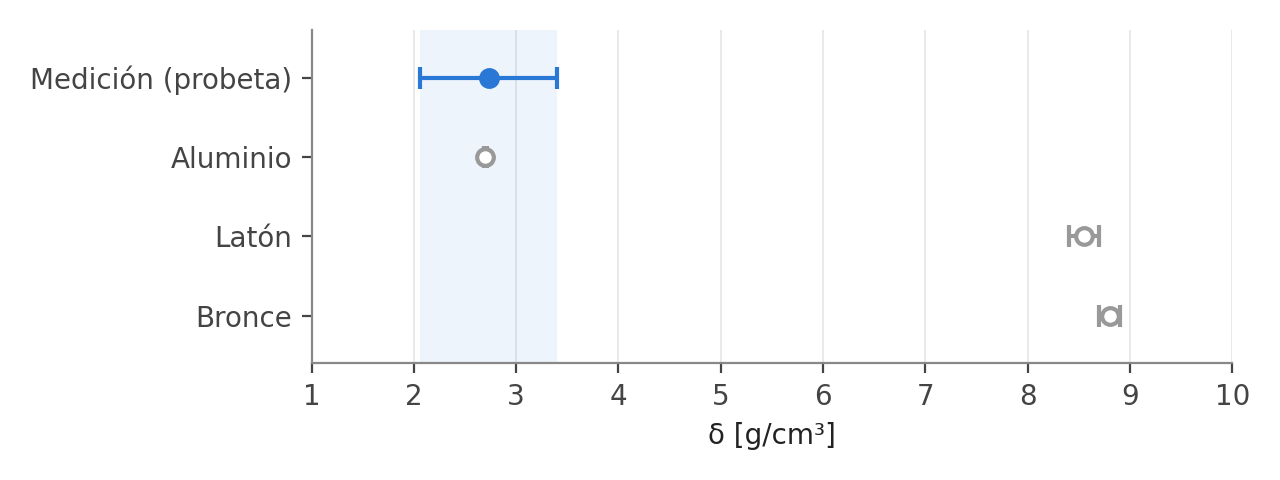
\includegraphics[width=0.72\textwidth]{fig1-densidad.png}
  \caption{Intervalo de la densidad medida comparado con valores tabulados de aluminio,
           latón y bronce.}
  \label{fig:densidad}
\end{figure}

\begin{figure}[htbp]
  \centering
  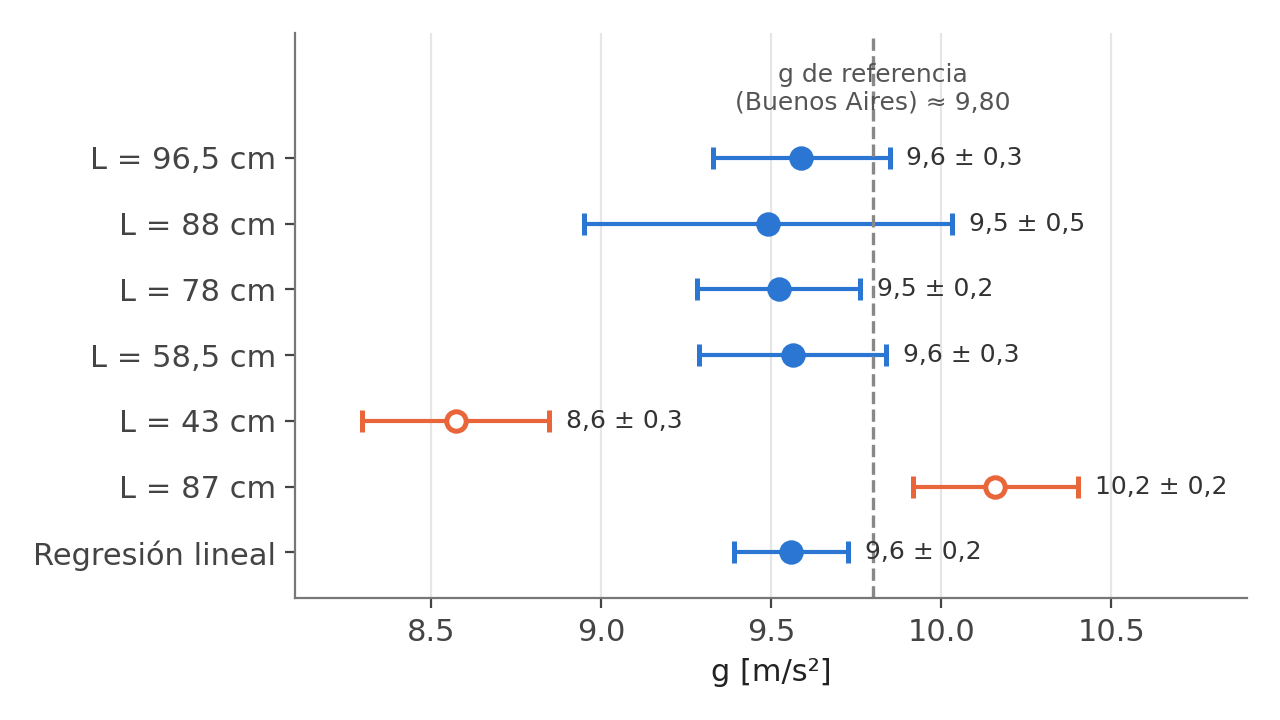
\includegraphics[width=0.72\textwidth]{fig2-gravedad.png}
  \caption{Valores de $g$ obtenidos para cada longitud y por regresión lineal, con sus
           intervalos de incerteza. En naranja, los puntos descartados.}
  \label{fig:gravedad}
\end{figure}

\begin{figure}[htbp]
  \centering
  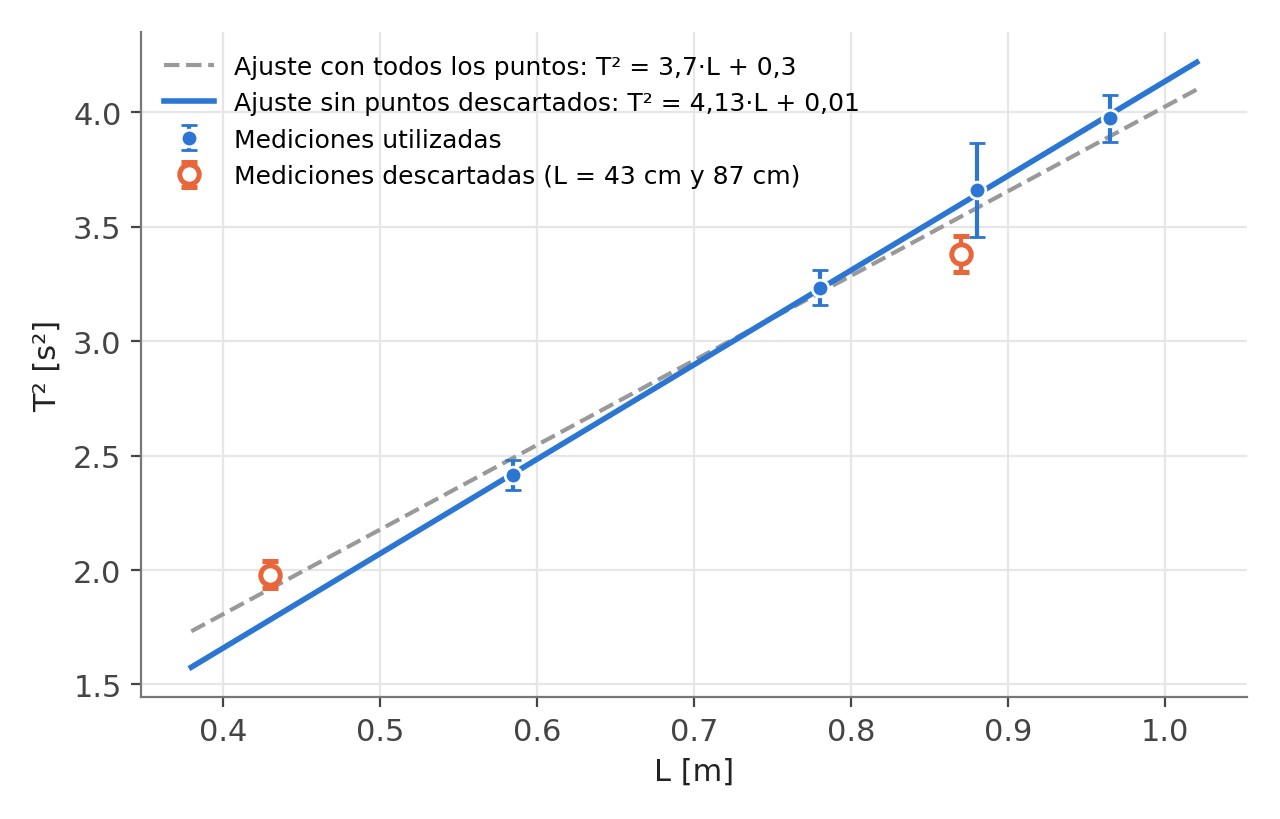
\includegraphics[width=0.72\textwidth]{fig3-regresion.png}
  \caption{$T^2$ en función de $L$ con ambos ajustes lineales. Las barras indican la
           incerteza de $T^2$; la de $L$ ($0{,}001$~m) es menor que el tamaño del punto.}
  \label{fig:regresion}
\end{figure}

% ------------------------------------------------------------------
\section{Análisis de resultados y conclusiones}

\subsection{Comparación entre el modelo y el sistema}
\paragraph{Densidad.} El intervalo obtenido, $[1{,}9\,;\,3{,}5]\ \mathrm{g/cm^3}$, contiene
la densidad del aluminio ($2{,}70\ \mathrm{g/cm^3}$), por lo que el cuerpo es compatible con
ese material. En cambio, las densidades del latón ($\approx 8{,}4$ a
$8{,}7\ \mathrm{g/cm^3}$) y del bronce ($\approx 8{,}7$ a $8{,}9\ \mathrm{g/cm^3}$) quedan muy
lejos del intervalo medido (Figura~\ref{fig:densidad}), por lo que se puede descartar que el
cuerpo esté hecho de alguno de ellos.

\paragraph{Aceleración de la gravedad.} Por el método directo se obtuvo
$g = (9{,}6 \pm 0{,}3)\ \mathrm{m/s^2}$ (3\%) y por regresión lineal
$g = (9{,}6 \pm 0{,}2)\ \mathrm{m/s^2}$ (2\%). Ambos intervalos se superponen, por lo
que las mediciones son comparables. Se elige como valor representativo el de la regresión
lineal, $\boldsymbol{g = (9{,}6 \pm 0{,}2)\ \mathbf{m/s^2}}$, ya que usa la información de
varias longitudes, tiene menor incerteza y es el único que no supera la cota del 2\%. Además,
en el ajuste sin los puntos anómalos la ordenada al origen resulta compatible con cero, como
predice el modelo, y el ajuste es casi perfecto ($R^2 = 0{,}9994$). Sin embargo, el
cumplimiento de la cota debe tomarse con reservas: el ajuste se basa en solo cuatro puntos,
tras descartar dos de los seis, y con la incerteza obtenida al propagar las barras de error
de $T^2$ el error relativo sería de alrededor del 7\%.

\subsection{Consecuencias de las discrepancias entre modelo y sistema}
Con un error relativo del 30\%, el intervalo de densidad también incluye otros materiales de
densidad similar (vidrio, granito, algunas cerámicas), así que la medición no alcanza para
identificar el material de forma unívoca. En el péndulo, los valores de $g$ quedan por
debajo del valor de referencia en Buenos Aires ($\approx 9{,}80\ \mathrm{m/s^2}$). Ambos
intervalos, $[9{,}3\,;\,9{,}9]\ \mathrm{m/s^2}$ por el método directo y
$[9{,}4\,;\,9{,}8]\ \mathrm{m/s^2}$ por regresión, lo contienen, pero el de la regresión solo
en su extremo superior: con los valores sin redondear, $[9{,}39\,;\,9{,}72]\ \mathrm{m/s^2}$,
no lo alcanzaría. Esto sugiere un error sistemático no contemplado. Por otro lado, al incluir los
dos puntos anómalos en el ajuste, la recta se inclina, la ordenada al origen se aleja de cero
y $g$ resulta muy por encima del valor esperado, con un error del 7\%.

\subsection{Hipótesis de esas discrepancias}
Para comparar el peso de cada fuente de error se calcularon los errores relativos de las
mediciones directas (Tabla~\ref{tab:errores}).

\begin{table}[htbp]
\centering
\small
\caption{Errores relativos de las mediciones directas según el instrumento utilizado.}
\label{tab:errores}
\begin{tabular}{llccc}
  \toprule
  \hdr{Magnitud} & \hdr{Instrumento} & \hdr{Valor típico} & \hdr{Incerteza} & \hdr{Error relativo} \\ \midrule
  Masa $m$      & Balanza    & 45,71 g  & 0,02 g  & 0,03 \% \\
  Volumen $V$   & Probeta    & 17 ml    & 5 ml    & 30 \%   \\
  Longitud $L$  & Regla      & 96,5 cm  & 0,1 cm  & 0,1 \%  \\
  Período $T$   & Cronómetro & 1,99 s   & 0,03 s  & 1 \%    \\
  \bottomrule
\end{tabular}
\end{table}

En la densidad, el error de la masa es despreciable frente al del volumen: prácticamente toda
la incerteza de $\delta$ proviene de la probeta, cuya incerteza de 5~ml es comparable al
volumen medido ($\approx 17$~ml). En el péndulo, el término dominante es el del período, que
además entra multiplicado por 2 en la expresión de $\Delta g/g$; el aporte de la longitud es
más de veinte veces menor.

La diferencia sistemática con el valor de referencia de $g$ puede deberse a que el modelo de
péndulo ideal supone una masa puntual, amplitudes pequeñas y rozamiento nulo, y a que la
longitud debe medirse hasta el centro de la esfera, lo cual no es sencillo con una regla.
También influye el tiempo de reacción al iniciar y detener el cronómetro, que no es igual en
cada medición: para $L = 96{,}5$~cm y $L = 88$~cm la dispersión entre las tres repeticiones
(hasta 1~s para $L = 88$~cm) superó la incerteza instrumental de 0,2~s, lo que muestra que
el tiempo de reacción real fue mayor a 0,2~s en algunas mediciones; en esos casos se adoptó
la incerteza obtenida de la dispersión. Los valores anómalos de 43~cm y
87~cm se atribuyen a errores groseros, probablemente en el registro de la longitud o en el
conteo de oscilaciones.

\subsection{Mejoras al método y dificultades en el desarrollo de la práctica}
Durante la práctica se descartaron las dos primeras tomas de volumen por errores durante la
medición, y las longitudes de 43~cm y 87~cm se excluyeron del ajuste final. Para mejorar el
resultado de la densidad convendría usar una probeta de menor diámetro y mayor resolución, un
cuerpo más voluminoso, o calcular el volumen geométricamente midiendo sus dimensiones con
calibre, lo que reduciría la incerteza del volumen varias veces. Para que el método directo
del péndulo cumpla la cota del 2\% con holgura habría que medir al menos unas 30
oscilaciones: con $\Delta t \approx 0{,}3$~s y $L = 96{,}5$~cm, $2\Delta T/T$ bajaría a
alrededor del 1\%. Se propone además hacer
más repeticiones por longitud, anotar los datos por duplicado para evitar errores de registro,
y usar un sensor o un video para medir el tiempo en lugar del cronómetro manual.

% ------------------------------------------------------------------
\section{Hoja de datos}
Mediciones registradas en el laboratorio el 16 de septiembre de 2026, tal como fueron
tomadas (sin procesar).

\begingroup
\small
\renewcommand{\arraystretch}{1.3}
\setlength{\aboverulesep}{0pt}\setlength{\belowrulesep}{0pt}
\newcolumntype{C}{>{\centering\arraybackslash}X}
\newcommand{\hojatitulo}[1]{%
  \par\vspace{14pt}\noindent{\color{fiuba}\rule[-2pt]{3pt}{11pt}}\hspace{6pt}%
  \textbf{#1}\par\vspace{5pt}}
\newcommand{\hojahdr}{\rowcolor{fiuba!10}}

\hojatitulo{Instrumentos y condiciones de medición}
\noindent
\begin{tabularx}{\textwidth}{@{\hspace{6pt}}l l X@{\hspace{6pt}}}
  \toprule
  \hojahdr \hdr{Instrumento} & \hdr{Apreciación} & \hdr{Observaciones} \\ \midrule
  Probeta graduada    & 2~ml    & Volumen por desplazamiento de agua \\
  Balanza electrónica & 0,01~g  & Masa del cuerpo \\
  Regla milimetrada   & 1~mm    & Longitud del péndulo, hasta el centro de la esfera \\
  Cronómetro digital  & 0,01~s  & Tiempo de reacción estimado: 0,2~s \\
  Transportador       & ---     & Amplitud inicial del péndulo: $10^\circ$ \\
  \bottomrule
\end{tabularx}

\noindent
\begin{minipage}[t]{0.485\textwidth}
  \hojatitulo{Parte 1: volumen (probeta)}
  \noindent
  \begin{tabularx}{\linewidth}{CCC}
    \toprule
    \hojahdr \hdr{Toma} & \hdr{$X_1$ [ml]} & \hdr{$X_2$ [ml]} \\ \midrule
    1 & 30 & 48 \\
    2 & 40 & 56 \\
    3 & 40 & 57 \\
    4 & 29 & 45 \\
    \bottomrule
  \end{tabularx}
\end{minipage}\hfill
\begin{minipage}[t]{0.485\textwidth}
  \hojatitulo{Parte 1: masa (balanza)}
  \noindent
  \begin{tabularx}{\linewidth}{CC}
    \toprule
    \hojahdr \hdr{Medición} & \hdr{$m$ [g]} \\ \midrule
    1 & 45,70 \\
    2 & 45,70 \\
    3 & 45,71 \\
    4 & 45,71 \\
    \bottomrule
  \end{tabularx}
\end{minipage}

\hojatitulo{Parte 2: péndulo (tiempo de $N = 10$ oscilaciones)}
\noindent
\begin{tabularx}{\textwidth}{CCCC}
  \toprule
  \hojahdr \hdr{Longitud $L$ [cm]} & \hdr{$t_1$ [s]} & \hdr{$t_2$ [s]} & \hdr{$t_3$ [s]} \\ \midrule
  96,5 & 20,10 & 19,60 & 20,10 \\
  88   & 19,77 & 18,91 & 18,72 \\
  78   & 18,20 & 17,96 & 17,79 \\
  58,5 & 15,71 & 15,43 & 15,48 \\
  43   & 13,92 & 14,12 & 14,18 \\
  87   & 18,21 & 18,50 & 18,45 \\
  \bottomrule
\end{tabularx}
\par
\endgroup

% ------------------------------------------------------------------
\section{Bibliografía utilizada}
\begin{enumerate}[label={[\arabic*]},leftmargin=2.5em]
  \item Facultad de Ingeniería, Universidad de Buenos Aires. \emph{Guía de presentación de
        informes de laboratorio}. Buenos Aires: FIUBA, 2018.
  % Verificar el título exacto y el año de la guía de la práctica.
  \item CB024 Física para Informática, Facultad de Ingeniería, Universidad de Buenos Aires.
        \emph{Guía de la práctica: Mediciones e Incertezas}. Buenos Aires: FIUBA, 2026.
  % Agregar la fuente de los valores tabulados de densidad utilizados.
\end{enumerate}

% ------------------------------------------------------------------
\section{Apéndices}
\label{sec:apendices}
\renewcommand{\thesubsection}{\alph{subsection})}
\renewcommand{\thesubsubsection}{\alph{subsection}.\arabic{subsubsection}}
\titleformat{\subsection}{\normalsize\bfseries}{\thesubsection}{0.6em}{}

\subsection{Cálculos realizados y propagación de incertezas}
\label{ap:calculos}

\subsubsection{Volumen del cuerpo}
La incerteza instrumental del volumen surge de propagar las incertezas de las dos lecturas:
\[
  V = X_2 - X_1, \qquad
  \Delta V_{\text{inst}} = \left|\frac{\partial V}{\partial X_1}\right| \Delta X_1
                         + \left|\frac{\partial V}{\partial X_2}\right| \Delta X_2
                         = \Delta X_1 + \Delta X_2 = 4\ \mathrm{ml}
\]
Esta es la apreciación con la que se obtiene cada valor de $V$. Aplicando la expresión para
mediciones repetidas a las cuatro tomas, con $V_M = 18$~ml y $V_m = 16$~ml:
\[
  \Delta V = \frac{(V_M + 4\ \mathrm{ml}) - (V_m - 4\ \mathrm{ml})}{2}
           = \frac{22\ \mathrm{ml} - 12\ \mathrm{ml}}{2} = 5\ \mathrm{ml}
  \quad\Rightarrow\quad
  V = (17 \pm 5)\ \mathrm{ml}
\]
Del mismo modo, para la masa:
$\Delta m = [(45{,}71 + 0{,}01) - (45{,}70 - 0{,}01)]/2\ \mathrm{g} = 0{,}015\ \mathrm{g}
\approx 0{,}02\ \mathrm{g}$, de modo que $m = (45{,}71 \pm 0{,}02)\ \mathrm{g}$. En los cálculos
que siguen se usan los valores sin redondear ($m = 45{,}705$~g, $\Delta m = 0{,}015$~g,
$V = 16{,}75$~ml).

\subsubsection{Densidad}
Aplicando la definición y propagando incertezas con derivadas parciales
(1~ml $=$ 1~cm$^3$):
\[
  \Delta\delta = \left|\frac{\partial\delta}{\partial m}\right| \Delta m
               + \left|\frac{\partial\delta}{\partial V}\right| \Delta V
               = \frac{1}{V}\,\Delta m + \frac{m}{V^2}\,\Delta V
\]
\[
  \delta = \frac{45{,}705\ \mathrm{g}}{16{,}75\ \mathrm{cm^3}} = 2{,}729\ \frac{\mathrm{g}}{\mathrm{cm^3}}
\]
\[
  \Delta\delta = \frac{0{,}015\ \mathrm{g}}{16{,}75\ \mathrm{cm^3}}
               + \frac{45{,}705\ \mathrm{g}}{\left(16{,}75\ \mathrm{cm^3}\right)^2} \cdot 5\ \mathrm{cm^3}
               = 0{,}0009 + 0{,}81 \approx 0{,}8\ \frac{\mathrm{g}}{\mathrm{cm^3}}
\]
Expresando la incerteza con una cifra significativa:
$\delta = (2{,}7 \pm 0{,}8)\ \mathrm{g/cm^3}$, con
$\varepsilon_\delta = 0{,}815 / 2{,}729 \approx 30\%$.

\subsubsection{Aceleración de la gravedad por método directo}
La incerteza instrumental del tiempo suma la resolución del cronómetro y el tiempo de
reacción, y se compara con la que surge de la dispersión de las tres repeticiones,
adoptándose la mayor:
\[
  \Delta t_{\text{inst}} = 0{,}01\ \mathrm{s} + 0{,}2\ \mathrm{s} = 0{,}21\ \mathrm{s},
  \qquad
  \Delta t_{\text{disp}} = \frac{(t_M + 0{,}01\ \mathrm{s}) - (t_m - 0{,}01\ \mathrm{s})}{2},
  \qquad
  \Delta t = \max(\Delta t_{\text{inst}}, \Delta t_{\text{disp}})
\]
\[
  \Delta T = \frac{\Delta t}{10},
  \qquad
  \Delta (T^2) = 2\,T\,\Delta T
\]
Para la longitud más larga, $L = 96{,}5$~cm ($t_M = 20{,}10$~s, $t_m = 19{,}60$~s,
$t_{\text{prom}} = 19{,}93$~s, $T = 1{,}993$~s):
\[
  \Delta t_{\text{disp}} = \frac{20{,}11\ \mathrm{s} - 19{,}59\ \mathrm{s}}{2} = 0{,}26\ \mathrm{s}
  > \Delta t_{\text{inst}}
  \quad\Rightarrow\quad
  \Delta T = 0{,}026\ \mathrm{s}
\]
\[
  g = \frac{4\pi^2 \cdot 0{,}965\ \mathrm{m}}{(1{,}993\ \mathrm{s})^2}
      = 9{,}59\ \frac{\mathrm{m}}{\mathrm{s^2}},
  \qquad
  \frac{\Delta g}{g} = \frac{0{,}1}{96{,}5} + 2 \cdot \frac{0{,}026}{1{,}993}
                     = 0{,}001 + 0{,}026 = 2{,}7\%
\]
de donde $\Delta g = 0{,}027 \cdot 9{,}59\ \mathrm{m/s^2} = 0{,}26\ \mathrm{m/s^2}$. Redondeando
la incerteza a una cifra significativa: $g = (9{,}6 \pm 0{,}3)\ \mathrm{m/s^2}$, con
$\varepsilon_g \approx 3\%$. El
mismo procedimiento se aplicó a las demás longitudes de la Tabla~\ref{tab:pendulo}.

\subsubsection{Aceleración de la gravedad por regresión lineal}
Con la pendiente del ajuste sin los puntos anómalos, $a = (4{,}13 \pm 0{,}07)\ \mathrm{s^2/m}$:
\[
  g = \frac{4\pi^2}{a} = \frac{4\pi^2}{4{,}13\ \mathrm{s^2/m}} = 9{,}56\ \frac{\mathrm{m}}{\mathrm{s^2}},
  \qquad
  \Delta g = \left|\frac{dg}{da}\right| \Delta a = \frac{4\pi^2}{a^2}\,\Delta a
           = 0{,}17\ \frac{\mathrm{m}}{\mathrm{s^2}}
\]
Redondeando la incerteza a una cifra significativa: $g = (9{,}6 \pm 0{,}2)\ \mathrm{m/s^2}$,
con $\varepsilon_g \approx 2\%$ (1,75\% sin redondear). Aquí $\Delta a$ es la incerteza de la pendiente por cuadrados mínimos, calculada a partir de
los residuos:
\[
  \Delta a = \sqrt{\frac{\sum_i \left(T_i^2 - a L_i - b\right)^2}{(n-2)\sum_i (L_i - \bar L)^2}},
  \qquad n = 4
\]
Si en cambio se ponderan los puntos con sus incertezas, $w_i = 1/\Delta(T_i^2)^2$, se obtiene
$\Delta a = 1/\sqrt{\sum_i w_i (L_i - \bar L_w)^2} \approx 0{,}3\ \mathrm{s^2/m}$ y
$\Delta g \approx 0{,}7\ \mathrm{m/s^2}$ (ver Sección~\ref{sec:resultados}).

\subsubsection{Recorte de $\boldsymbol{\pi}$}
Siguiendo el criterio de la guía, el error cometido al recortar $\pi$ debe ser al menos diez
veces menor que el menor error relativo de las mediciones.
En el cálculo de $g$ intervienen $L$ y $T$; el menor error relativo es el de la longitud,
$\varepsilon_L = 0{,}1/96{,}5 \approx 0{,}1\%$. Como $\pi$ aparece al cuadrado, aporta
$2\,\varepsilon_\pi$ al error relativo de $g$:
\[
  2\,\varepsilon_\pi \leq \frac{1}{10}\,\varepsilon_L = 0{,}01\%
  \quad\Rightarrow\quad
  \varepsilon_\pi \leq 0{,}005\%
\]
Tomar $\pi = 3{,}14$ ($\varepsilon_\pi \approx 0{,}05\%$) o $\pi = 3{,}142$
($\varepsilon_\pi \approx 0{,}01\%$) no cumpliría el criterio. En los cálculos se usó
$\pi = 3{,}1416$, con $\varepsilon_\pi \approx 0{,}0002\%$, que sí lo cumple.

\end{document}
